\documentclass[notes]{beamer} 
%\usepackage{pgfpages}
%\setbeameroption{show notes on second screen=right}
\usepackage[british]{babel}
\usepackage{graphicx,hyperref,ru,url}
\usepackage{listings}
\usepackage{xcolor}

\definecolor{red}{RGB}{190,49,26}
\title[Application Lifecycle Management]{Application Lifecycle Management}
\subtitle{An overview of existing tools}


\author[Pedro Tavares]{%
  \texorpdfstring{%
    \begin{columns}
      \column{.4\linewidth}
      \centering
      Pedro Tavares \\ \texttt{up201708899@fe.up.pt}
    \end{columns}
 }
 {Pedro Tavares}
}

\institute[Faculty of Engineering of the University of Porto]{Faculty of Engineering of the University of Porto}

\date[MESW1718-PPES]{15 December 2017}

\begin{document}

\begin{frame}
  \titlepage
\end{frame}

\section{Introduction}

\begin{frame}
  \frametitle{Application Lifecycle Management}
  \setbeamercovered{transparent}
  \begin{definition}[Application Lifecycle Management]<1->
  Is the product lifecycle management of software.
  \end{definition}
  \begin{block}{}<2->
  It covers the entire lifecycle from the \textbf{idea conception}, through to the \textbf{development}, \textbf{testing}, \textbf{deployment}, \textbf{support} and ultimately \textbf{retirement} of systems.
  \end{block}
  \begin{block}{}<3->
  Consists in three core aspects: \textbf{governance}, \textbf{development}, and \textbf{operations}.
  \end{block}
\end{frame}

\begin{frame}
  \frametitle{Application Lifecycle Management}
  \begin{figure}
    \centering
    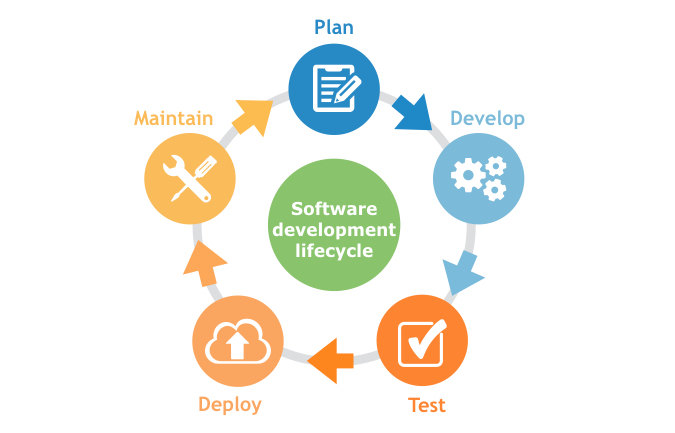
\includegraphics[scale=0.35]{alm.png}
    \caption{ALM should cover every stage of Software Development Lifecycle.}
  \end{figure}
\end{frame}

\section{Core Aspects of ALM}

\begin{frame}
  \frametitle{Core Aspects of ALM}
  \setbeamercovered{transparent}
  \begin{itemize}[<+->]
  \item \textbf{Governance}: extends over the entire application lifecycle to make sure the application always provides what the business needs;
  \item \textbf{Development}: occurs in the first part of an application’s lifecycle, then happens periodically as
the application is updated;
  \item \textbf{Operations}: begins shortly before an application is deployed, then continues until the application is removed from service.
  \end{itemize}
\end{frame}

\begin{frame}
  \frametitle{Why the need of ALM Tools?}
  \centering
  \textit{"More and more software development companies realize that relying on inadequate legacy tools and loads of manual work is no longer feasible."}
\end{frame}

\section{Why the need of ALM Tools?}

\begin{frame}
  \frametitle{Why the need of ALM Tools?}
  \setbeamercovered{transparent}
  Companies realized that with proper ALM tooling they can have integrated teams that: \\
  \begin{itemize}[<+->]
  \item \textbf{Collaboratively} define \textbf{software requirements};
  \item Plan \textbf{sprints} and \textbf{releases};
  \item \textbf{Test} the product \textbf{during development};
  \item \textbf{Continuously deploy} the latest product updates.
  \end{itemize}
\end{frame}

\begin{frame}
  \frametitle{The problem of most ALM tools}
  \setbeamercovered{transparent}
  \begin{itemize}[<+->]
  \item GitHub follow a \textbf{marketplace strategy} where other vendors cover most of the product categories;
  \item Atlassian covers most of the product categories but the user or \textbf{reseller has to integrate} them together;
  \item Requires \textbf{multiple applications} to cover the ALM stages.
  \end{itemize}
\end{frame}

\section{The single application}

\begin{frame}
  \begin{figure}
    \frametitle{GitLab: The single application}
    \centering
    
\includegraphics[scale=0.3]{gitlab.png}\\
    \textit{"GitLab is a single application that does} \\
    \textit{everything from planning to monitoring."}
  \end{figure}
\end{frame}

\begin{frame}
  \frametitle{Advantages of a single application}
  \setbeamercovered{transparent}
  \begin{itemize}[<+->]
  \item \textbf{\textit{Single}} Authentication/Authorization;
  \item \textbf{\textit{Single}} Project/Setup;
  \item \textbf{\textit{Single}} Interface/Data-Store/Overview;
  \item \textbf{\textit{Single}} Vendor;
  \end{itemize}
\end{frame}

\section{GitLab Features}

\begin{frame}
 \frametitle{GitLab Features}
 \setbeamercovered{transparent}
 \begin{itemize}[<+->]
    \item \textbf{\textit{Planning}} Issue tracking	and Kanban boards;
    \item \textbf{\textit{Creating}} Version control and Code reviews;   
    \item \textbf{\textit{Verifying}} Continuous integration;
    \item \textbf{\textit{Releasing}} Continuous deployment;
    \item \textbf{\textit{Monitoring}};
  \end{itemize}
\end{frame}

\begin{frame}
  \begin{figure}
    \frametitle{Planning: GitLab Issues (Issue tracking)}
    \centering
    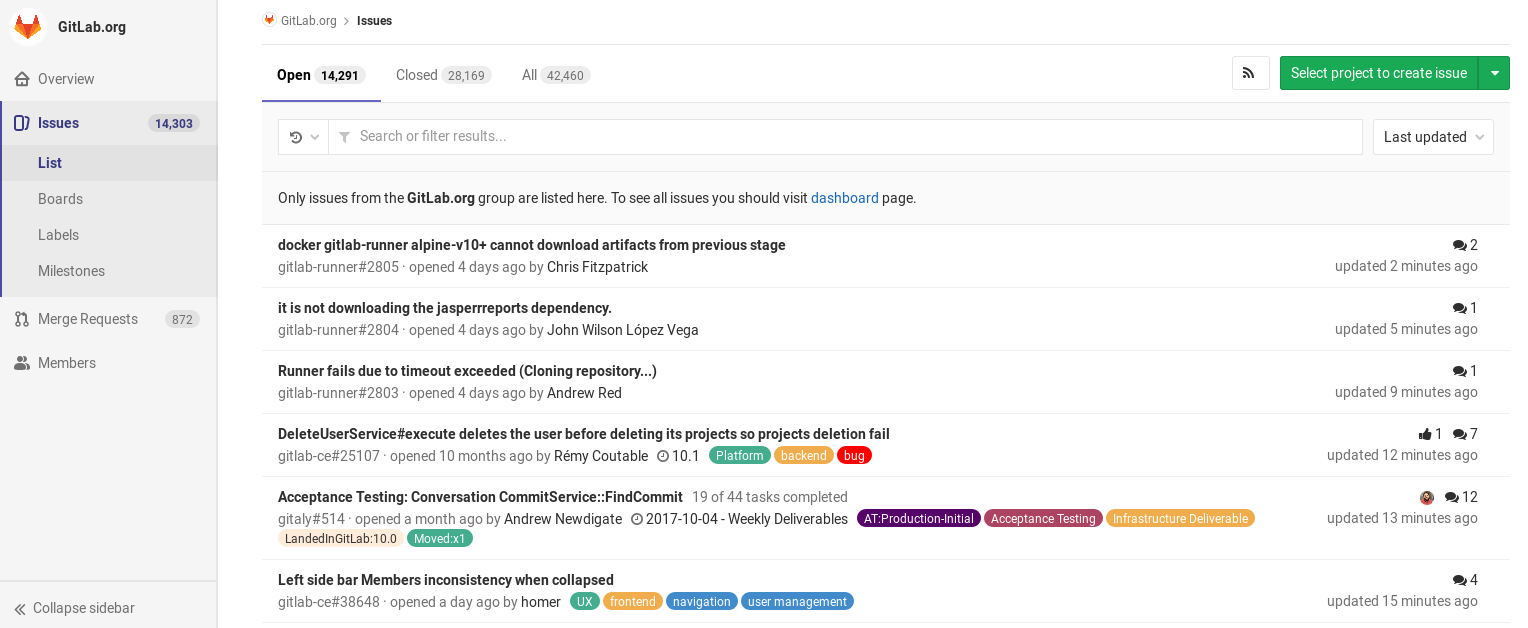
\includegraphics[scale=0.2]{issues.png}
  \end{figure}
\end{frame}

\begin{frame}
  \begin{figure}
    \frametitle{Planning: GitLab Boards (Kanban boards)}
    \centering
    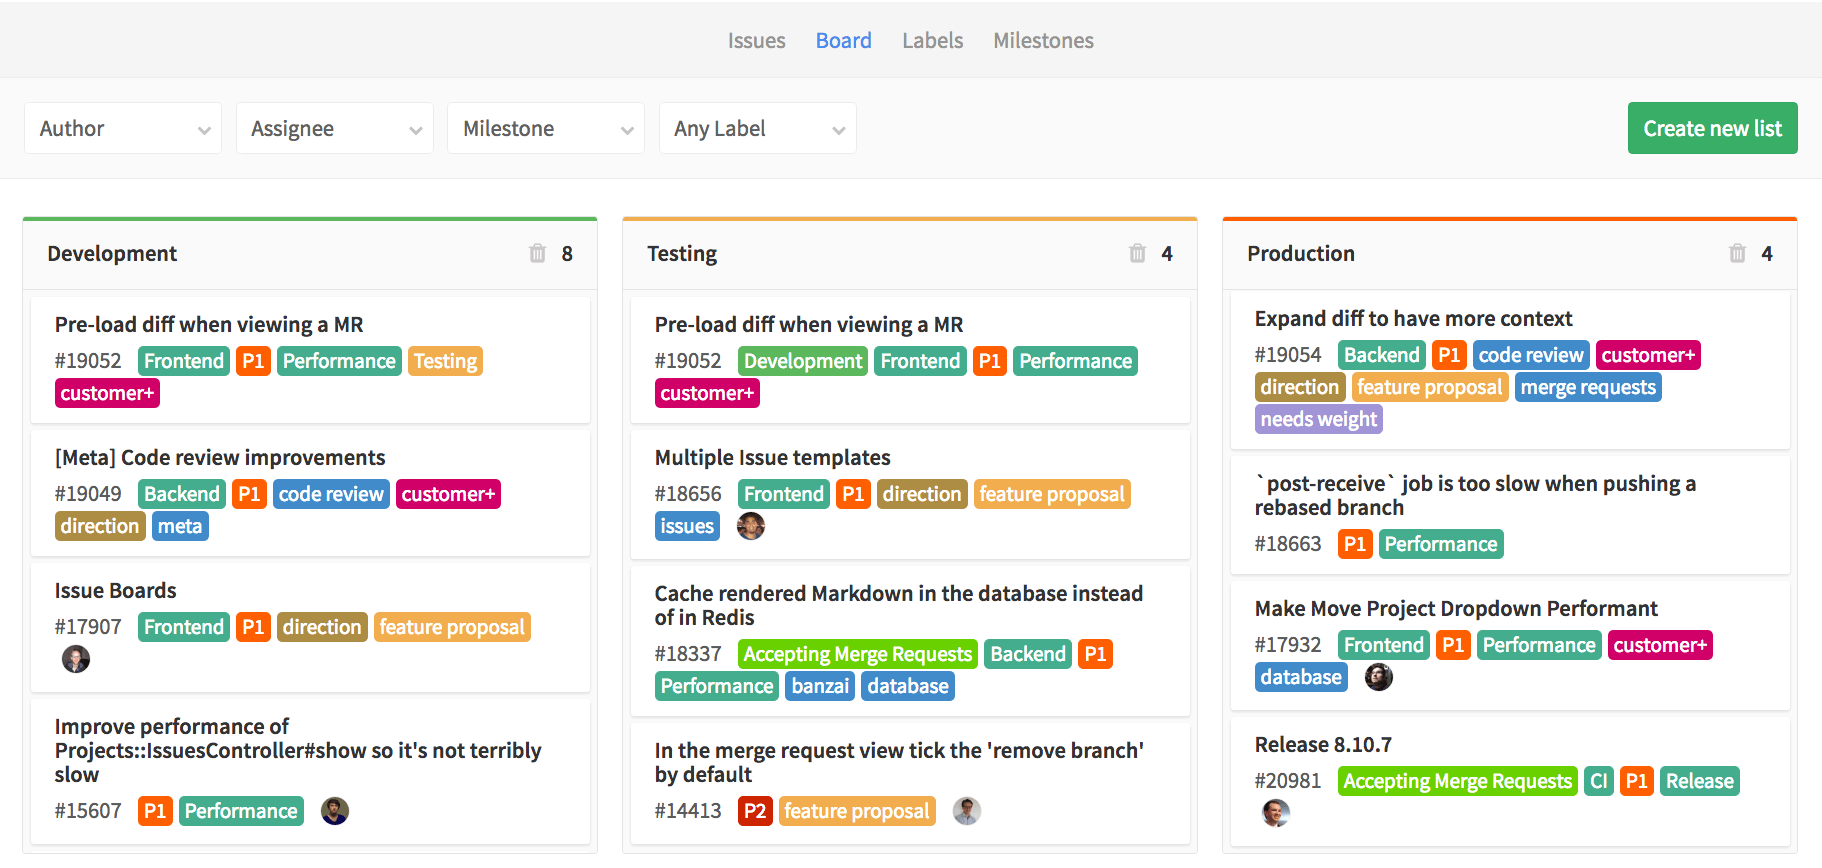
\includegraphics[scale=0.165]{boards.png}
  \end{figure}
\end{frame}

\begin{frame}
  \begin{figure}
    \frametitle{Creating: GitLab SCM (Version control)}
    \centering
    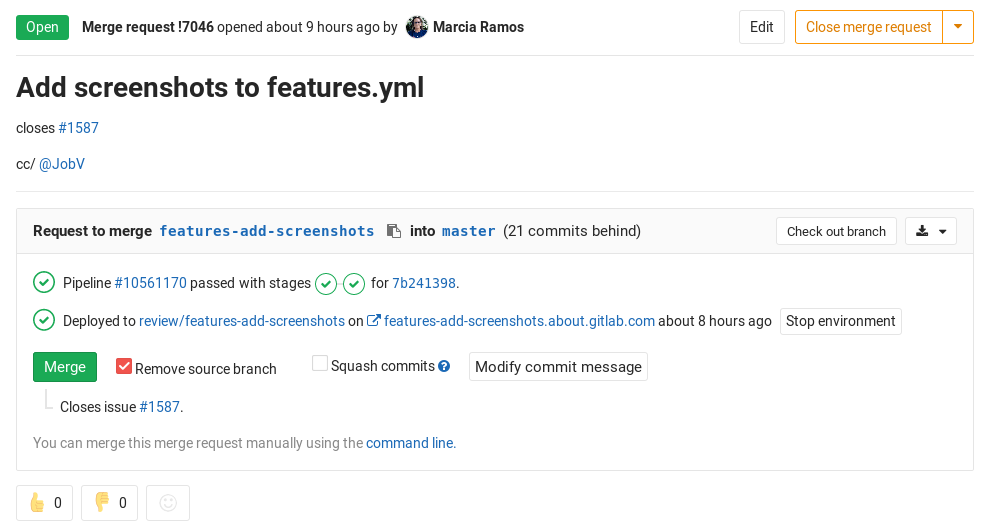
\includegraphics[scale=0.3]{version-control.png}
  \end{figure}
\end{frame}

\begin{frame}
  \begin{figure}
    \frametitle{Creating: GitLab SCM (Code review)}
    \centering
    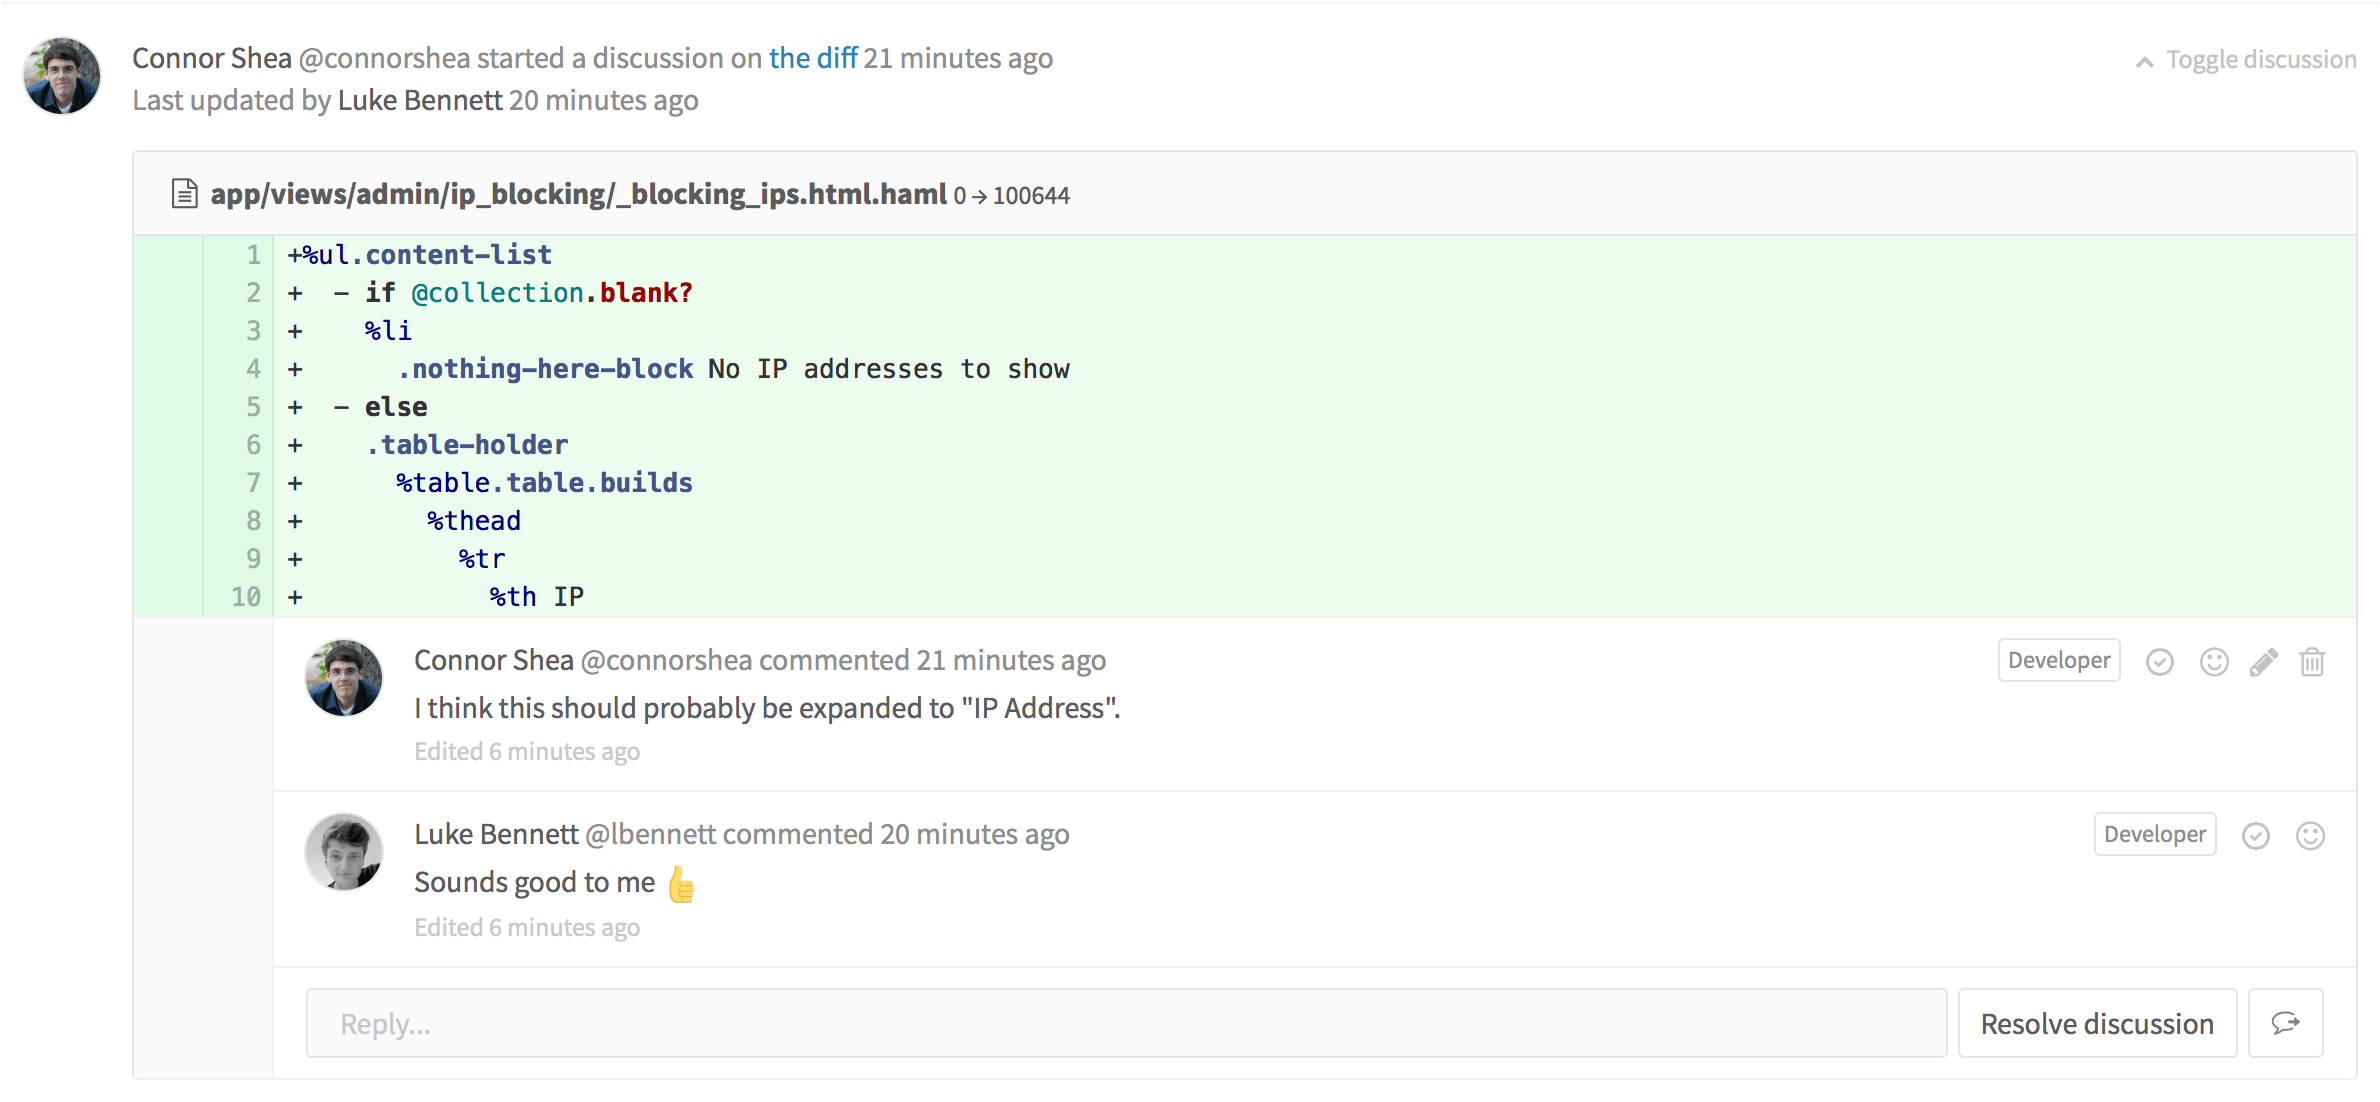
\includegraphics[scale=0.25]{code-review.png}
  \end{figure}
\end{frame}

\begin{frame}
  \begin{figure}
    \frametitle{Verifying: GitLab CI (Continuous integration)}
    \centering
    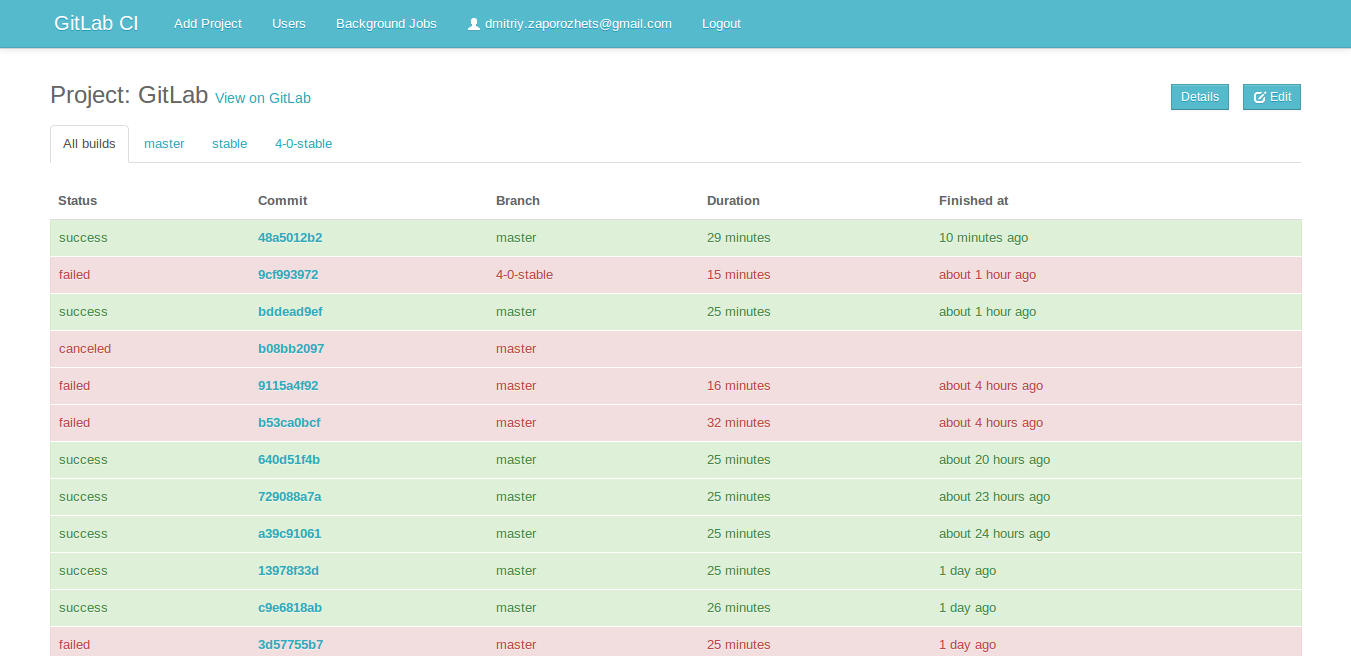
\includegraphics[scale=0.2]{ci.png}
  \end{figure}
\end{frame}

\begin{frame}
  \begin{figure}
    \frametitle{Releasing: GitLab CD (Continuous deployment)}
    \centering
    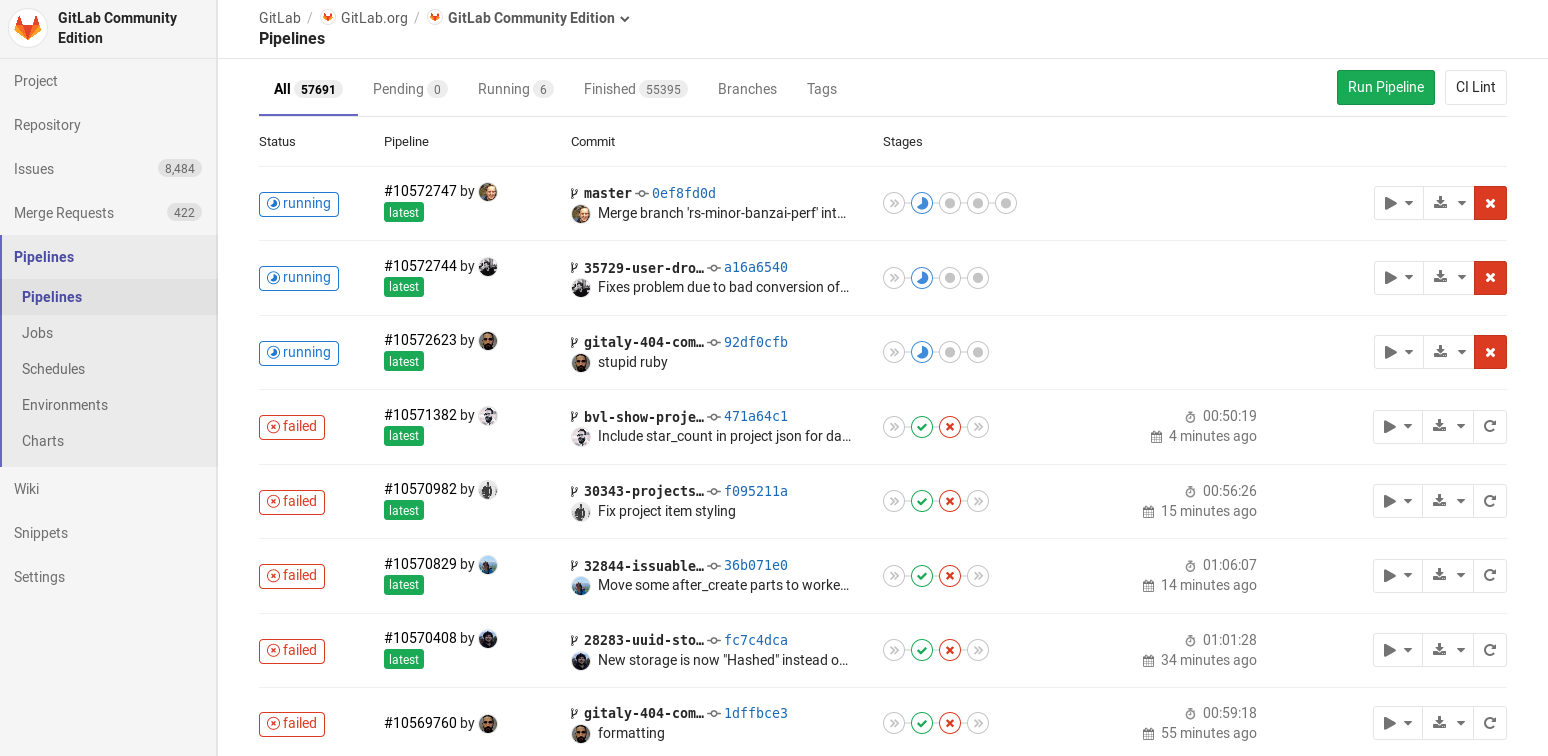
\includegraphics[scale=0.165]{cd.png}
  \end{figure}
\end{frame}

\begin{frame}
  \begin{figure}
    \frametitle{Monitoring: GitLab Metrics}
    \centering
    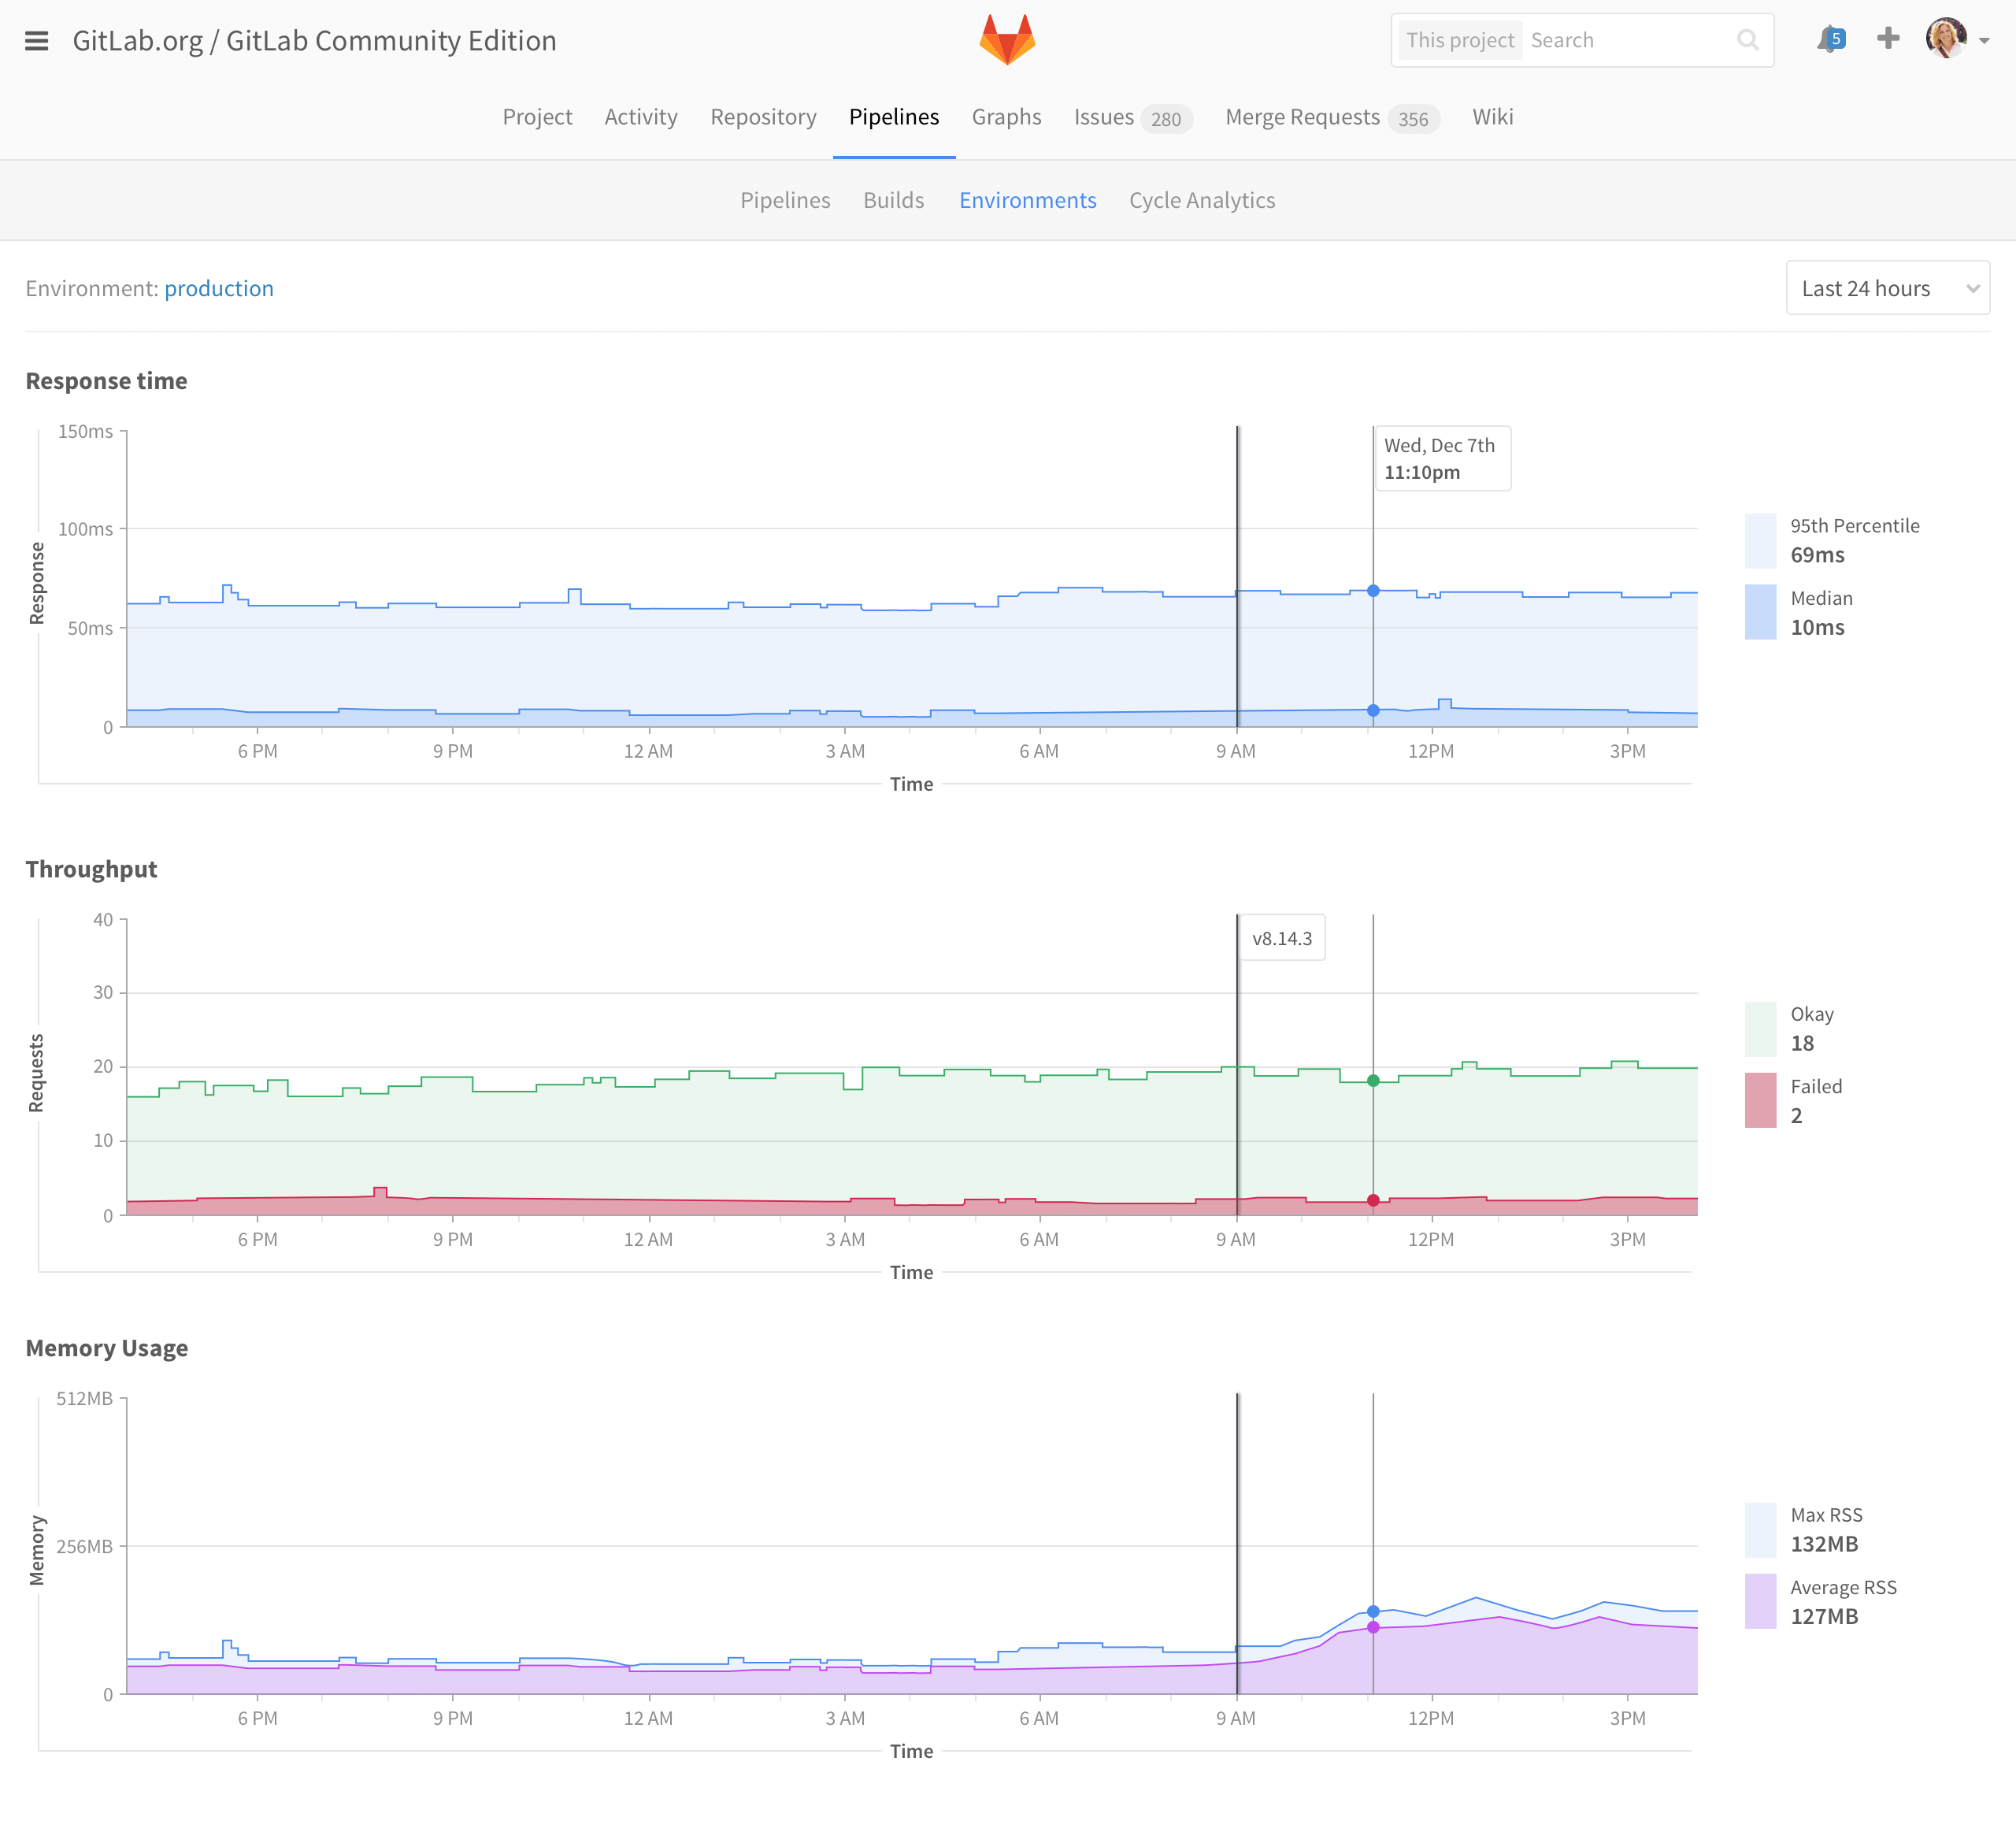
\includegraphics[scale=0.10]{monitoring.png}
  \end{figure}
\end{frame}

\begin{frame}
  \titlepage
\end{frame}

\end{document}
